\subsection{Control Unit}

\begin{figure}[h]
    \centering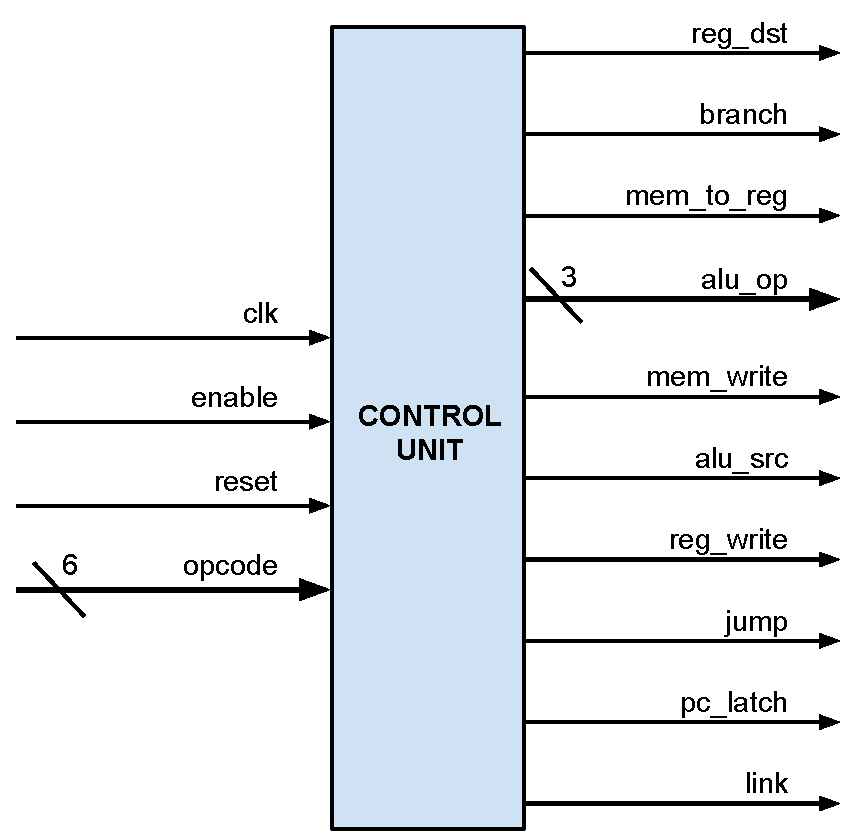
\includegraphics[scale=0.5]{figures/control_unit_block_symbol}
    \caption{Control Unit block symbol}
    \label{figure:ctrl_unit_block_symbol}    
\end{figure}
The control unit is in many ways the brain within our processor implementation. It is responsible for controlling how the data path behaves during the execution of the program. It does so by controlling a total of 10 different control signals. Figure~\ref{figure:ctrl_unit_block_symbol} shows a black box diagram of the control unit with only the input and output signals.

In essence it is implemented as two parts, a synchronous state machine that updates the internal state of the control unit, and is an essenstial part of a multi cycle design. The second, sequential, part is responsible for driving most control signals and is explained in detail later. The state machine have 4 possible states, RESET, FETCH, EXECUTE and STALL. Figure~\ref{figure:ctrl_unit_state_machine} shows the four states, the transition conditions and the effect the transitions have on the {\bf pc\_latch} control signal. In an effort to keep the figure as simple as possible the fact that transitions happen only on the rising edge of the clock cycle and only if the enable signal is asserted has been hidden from the transition conditions.


\begin{figure}[h]
    \centering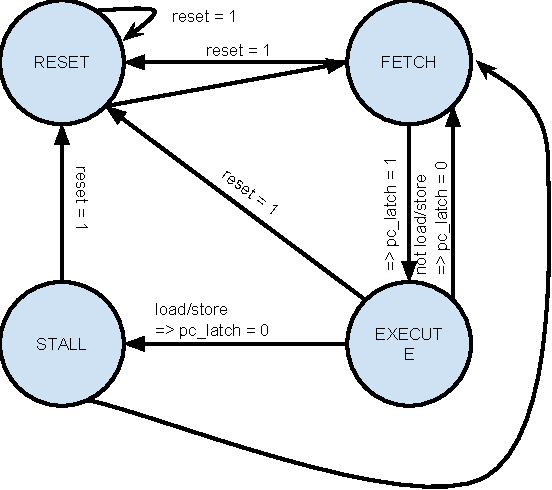
\includegraphics[scale=0.8]{figures/control_unit_state_machine}
    \caption{Control Unit state machine}
    \label{figure:ctrl_unit_state_machine}    
\end{figure}

The RESET state is a special state the processor only enters when the reset signal is asserted, it is also the default state of the processor before it starts. It should be noted that the reset transitions have a higher priority than the others, hence if the reset signal is high the unit is forced into the RESET state.

The FETCH state is where the control unit is waiting for the next instruction to be fetched from the instruction memory. Upon entering this state from any other state than RESET the control signal {\bf pc\_latch} is asserted, signaling that the PC register should latch its next value. The reason why latching is not done when coming from RESET is because the PC at that point is zero, toggling the {\bf pc\_latch} would make it increment to 1 and hence always skipping the first instruction. As the instruction memory is synchronous the next instruction is available on the next rising clock edge, and therefore the transition to EXECUTE is conditionless.

The EXECUTE state is where the work is done, upon entering this state the instruction word is ready, and the control unit has to decode it and drive all the control signals to their correct value. This decoding is done by the sequential part of the control unit. On the next clock edge the control unit enters either STALL or EXECUTE depending on whether or not the instruction being executed has to access the data memory. If the instruction does access data memory we need to stall for a cycle and the transtion to STALL is taken, if not the control unit enters FETCH again.

The STALL state does nothing but holding the control signals asserted by EXECUTE, this is because the data memory is synchronous as well and after setting up the data path in EXECUTE we need to wait an additional clock cycle before the data has been written or the data to be read is available on the data out bus from the data memory. From STALL there is a conditonless transition back to FETCH.

The second part of the control unit is a sequential circuit that based on the current internal state of the unit as well as the current opcode drives the control signals. An overview of the inputs and corresponding outputs can be found in table~\ref{table:control_signals}. In the table a dash indicates a don't care value, for output signals this indicates that the value that is already set will be hold in the given state. A more indepth explanation of what the different control singals do is given in the section covering the overall processor architecture. The most important thing to note in this table is that in the FETCH state all destructive singals, signals that will cause data to be written, is pulled low. This is really important because upon entering EXECUTE the datapath will be unstable while signals propagate, and if a destrutive signal is high at that point invalid data might be written to the registers or the memory. 


\begin{table}[h]
	\begin{tabular}{l|l|l|l|l|l|l|l|l|l|l|l}
    \swtext{State} & \swtext{Opcode} & \swtext{reg\_dst} & \swtext{branch}  & \swtext{mem\_to\_reg} & \swtext{alu\_op} & \swtext{mem\_write} & \swtext{reg\_write} & \swtext{alu\_src} & \swtext{jump} & \swtext{link} & \swtext{next\_state} \\

    \hline
    FETCH   & ------  & - & - & - & -                & 0 & 0 & - & - & - & EXECUTE \\ 
    \hline
    EXECUTE & 000000 (ALU) & 1 & 0 & 0 & FUNC        & 0 & 1 & 0 & 0 & 0 & FETCH \\ 
            & 100011 (LW)  & 0 & 0 & 1 & LOAD\_STORE & 0 & 1 & 1 & 0 & 0 & STALL \\
            & 101011 (SW)  & 0 & 0 & 1 & LOAD\_STORE & 1 & 0 & 1 & 0 & 0 & STALL \\  
            & 001111 (LUI) & 0 & 0 & 1 & LDI         & 0 & 1 & 1 & 0 & 0 & FETCH \\
            & 000100 (BEQ) & 1 & 1 & 0 & BRANCH      & 0 & 0 & 0 & 0 & 0 & FETCH \\  
            & 000010 (J)   & 1 & 0 & 0 & BRANCH      & 0 & 0 & 0 & 1 & 0 & FETCH \\ 
            & 000011 (JAL) & 1 & 0 & 0 & BRANCH      & 0 & 0 & 0 & 1 & 1 & FETCH \\
            & XXXXXX (Undef) & 0 & 0 & 0 & FUNC & 0 & 0 & 0 & 0 & 0 & FETCH \\
    \hline
    STALL   & ------ & - & - & - & - & - & - & - & - & - & FETCH \\
    \hline
    RESET   & ------ & 0 & 0 & 0 & FUNC & 0 & 0 & 0 & 0 & 0 & FETCH \\
    \hline
    \end{tabular}

    \caption{Mapping between control signals, internal state and the opcode}
    \label{table:control_signals}
\end{table}
